\chapter{Metodologia}\label{cap:metodologia}

% \MexerDepois{Escrever algo aqui}

Neste capítulo, são explorados os métodos utilizados para a construção do trabalho proposto, inicialmente com uma apresentação geral e em seguida com uma apresentação detalhada.

\section{Abordagem}

A abordagem utilizada no sistema consiste em, inicialmente, carregar o arquivo de imagem correspondente à foto do remédio a ser buscado.
Dessa imagem, são geradas versões em diferentes codificações de cores, e cada uma tem suas componentes analisadas.

A análise de cada versão resulta numa lista de termos textuais, que serão organizados e buscados no sistema do Bulário Eletrônico da \ac{Anvisa} \cite{anvisa2020bulario}.

Se um dos termos buscado for encontrado com sucesso, será carregado o arquivo digital da bula deste medicamento.
A \autoref{fig:fluxograma} apresenta o fluxograma geral do funcionamento do sistema.

\begin{figure}[htbp]
    \centering
    % 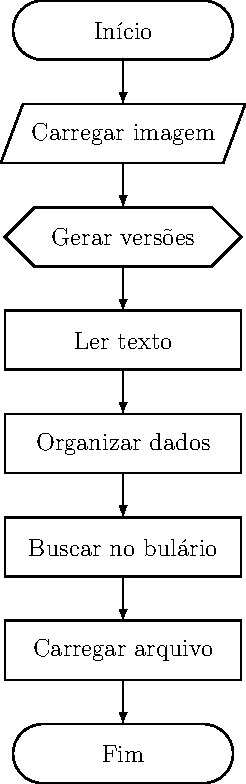
\includegraphics{../pictures/fluxograma_0.pdf}
    \caption{Fluxograma geral do funcionamento.}
    % https://www.youtube.com/watch?v=e968B1PwIbs&list=PLkRY1UknxTS0exb3ccUBJS1_e0TlSozFW&index=2

\begin{tikzpicture}[node distance=1.5cm]
    \node (s) [startstop] {Início};
    \node (a1) [below of=s, io] {Carregar imagem};
    \node (a2) [below of=a1, process] {Gerar versão};
    \node (a3) [below of=a2, process] {Ler texto};
    \node (a4) [below of=a3, loop] {Há outra versão?};
    \node (a5) [below of=a4, process] {Organizar dados};
    \node (a6) [below of=a5, process] {Buscar no bulário};
    \node (a7) [below of=a6, process] {Carregar arquivo};
    \node (f)  [below of=a7, startstop] {Fim};

    \node [left of=a1, auxBlockPhantom] {\phantom{\autoref{ssec:carregar}}};

    \node [right of=a1, auxBlock] {\autoref{ssec:carregar}};
    \node [right of=a2, auxBlock] {\autoref{ssec:versoes}};
    \node [right of=a3, auxBlock] {\autoref{ssec:ler}};
    \node [right of=a5, auxBlock] {\autoref{ssec:organizar}};
    \node [right of=a6, auxBlock] {\autoref{ssec:buscar}};
    \node [right of=a7, auxBlock] {\autoref{ssec:arquivo}};

    \draw [niceBrace] ([yshift=0.6cm, xshift=2.25cm]a1.center) -- ([yshift=-0.6cm, xshift=2.25cm]a1.center);
    \draw [niceBrace] ([yshift=0.6cm, xshift=2.25cm]a2.center) -- ([yshift=-0.6cm, xshift=2.25cm]a2.center);
    \draw [niceBrace] ([yshift=0.6cm, xshift=2.25cm]a3.center) -- ([yshift=-0.6cm, xshift=2.25cm]a3.center);
    \draw [niceBrace] ([yshift=0.6cm, xshift=2.25cm]a5.center) -- ([yshift=-0.6cm, xshift=2.25cm]a5.center);
    \draw [niceBrace] ([yshift=0.6cm, xshift=2.25cm]a6.center) -- ([yshift=-0.6cm, xshift=2.25cm]a6.center);
    \draw [niceBrace] ([yshift=0.6cm, xshift=2.25cm]a7.center) -- ([yshift=-0.6cm, xshift=2.25cm]a7.center);

    \node [anchor=north west, font = {\scriptsize\bfseries}, Red] at (a4.south) {N};
    \node [anchor=south east, font = {\scriptsize\bfseries}, Green] at (a4.west) {S};

    % \node [fit=(a1)] (fita1) {}; \draw [niceBrace] ([yshift=2.5pt]fita1.north east) -- ([yshift=-2.5pt]fita1.south east);
    % \node [fit=(a2)] (fita2) {}; \draw [niceBrace] ([yshift=2.5pt]fita2.north east) -- ([yshift=-2.5pt]fita2.south east);
    % \node [fit=(a3)] (fita3) {}; \draw [niceBrace] ([yshift=2.5pt]fita3.north east) -- ([yshift=-2.5pt]fita3.south east);
    % \node [fit=(a5)] (fita5) {}; \draw [niceBrace] ([yshift=2.5pt]fita5.north east) -- ([yshift=-2.5pt]fita5.south east);
    % \node [fit=(a6)] (fita6) {}; \draw [niceBrace] ([yshift=2.5pt]fita6.north east) -- ([yshift=-2.5pt]fita6.south east);
    % \node [fit=(a7)] (fita7) {}; \draw [niceBrace] ([yshift=2.5pt]fita7.north east) -- ([yshift=-2.5pt]fita7.south east);


    \draw [arrow] (s) -- (a1);
    \draw [arrow] (a1) -- (a2);
    \draw [arrow] (a2) -- (a3);
    \draw [arrow] (a3) -- (a4);
    \draw [arrow] (a4) -- (a5);
    \draw [arrow] (a4) -- ([xshift=-.5cm]a4.west) |- (a2);
    \draw [arrow] (a5) -- (a6);
    \draw [arrow] (a6) -- (a7);
    \draw [arrow] (a7) -- (f);
\end{tikzpicture}
% \begin{tikzpicture}[node distance=1.5cm]
%     \node (s) [startstop] {Início};
%     \node (a1) [below of=s, io] {Carregar imagem};
%     \node (a2) [below of=a1, loop] {Gerar versões};
%     \node (a3) [right of=a1, node distance=5cm, process] {Ler texto};
%     \node (a5) [below of=a3, process] {Organizar dados};
%     \node (a6) [right of=a3, node distance=5cm, process] {Buscar no bulário};
%     \node (a7) [below of=a6, process] {Carregar arquivo};
%     \node (f)  [below of=a7, startstop] {Fim};

%     \draw [arrow] (s) -- (a1);
%     \draw [arrow] (a1) -- (a2);
%     \draw [arrow] (a2) -| ($(a2)!0.5!(a3)$) |- (a3);
%     \draw [arrow] (a3) -- (a5);
%     \draw [arrow] (a5) -| ($(a5)!0.5!(a6)$) |- (a6);
%     \draw [arrow] (a6) -- (a7);
%     \draw [arrow] (a7) -- (f);
% \end{tikzpicture}
% \begin{tikzpicture}[node distance=1.5cm]
%     \node (s) [startstop] {Início};
%     \node (a1) [below of=s, io] {Carregar imagem};
%     \node (a2) [right of=a1, node distance=5cm, loop] {Gerar versões};
%     \node (a3) [right of=a2, node distance=5cm, process] {Ler texto};
%     \node (a5) [below of=a1, node distance=2cm, process] {Organizar dados};
%     \node (a6) [right of=a5, node distance=5cm, process] {Buscar no bulário};
%     \node (a7) [right of=a6, node distance=5cm, process] {Carregar arquivo};
%     \node (f)  [below of=a7, startstop] {Fim};

%     \draw [arrow] (s) -- (a1);
%     \draw [arrow] (a1) -- (a2);
%     \draw [arrow] (a2) -- (a3);
%     \draw [arrow] (a3) |- ($(a3)!0.5!(a5)$) -| (a5);
%     \draw [arrow] (a5) -- (a6);
%     \draw [arrow] (a6) -- (a7);
%     \draw [arrow] (a7) -- (f);
% \end{tikzpicture}
    \caption*{Fonte: Autor.}
    \label{fig:fluxograma}
\end{figure}

\section{Detalhamento}

Nesta seção, serão detalhados os métodos utilizados em cada passo da análise da imagem.

\subsection{Carregar arquivo de imagem}\label{ssec:carregar}

O primeiro passo no processo de análise consiste em carregar a imagem do arquivo escolhido, para isso, foi utilizada a função \textit{imread}, da biblioteca de processamento de imagem \textit{OpenCV}.

Essa função retorna os dados da imagem como um tensor no formato \acs{BGR} \cite{CV2imread}.
Em seguida, a imagem é convertida para o formato \ac{RGB} e é dado início ao processo de leitura do texto na imagem.

O \autoref{cod:carregar} apresenta a simplificação do bloco de código responsável por realizar essa ação.

\begin{lstfloat}[htbp]
    \centering
    \lstinputlisting[label=cod:carregar, caption={Carregar arquivo de imagem, simplificado.}]{../code/ex_carregar.py}
    \caption*{Fonte: Autor.}
\end{lstfloat}

\subsection{Realizar leitura do texto na imagem}\label{ssec:ler}

O processamento do texto presente na imagem é realizado através do motor de \ac{OCR} \textit{Tesseract OCR}, sendo interfaceado pela função \textit{image\_to\_data} da biblioteca \textit{pytesseract}, desenvolvida para facilitar o uso deste motor em Python \cite{samuelhoffstaetter2024, tesseract2024}.
O \autoref{cod:ler} apresenta uma simplificação da primeira parte do bloco de código associado a leitura dos termos.

\begin{lstfloat}[htbp]
    \centering
    \lstinputlisting[label=cod:ler, caption={Ler texto da imagem, simplificado.}]{../code/ex_ler.py}
    \caption*{Fonte: Autor.}
\end{lstfloat}


Essa função retorna a lista de termos encontrados, junto de informações adicionais a respeito, como confiabilidade e coordenadas da caixa que envolve o termo na imagem \cite{samuelhoffstaetter2024}.
As informações adicionais são utilizadas para filtrar e posteriormente classificar a ordem de prioridade da análise dos termos encontrados.

A filtragem realizada nesta etapa consiste em descartar termos com confiabilidade abaixo de \SI{10}{\percent} ou área menor que um parâmetro padrão.
A área mínima é relativa ao tamanho da imagem, em quantidade de \acp{pixel}, dado pela \autoref{eq:area_minima}, calculado pelo piso dos produtos de \SI{2}{\percent} das dimensões totais da imagem.
A \autoref{fig:fotos:tamanho} apresenta um exemplo da área mínima que um termo deve ocupar para ser considerado.
O \autoref{cod:ler:2} apresenta a continuação da lógica simplificada envolvida nessa seção.

\begin{equation}\label{eq:area_minima}
    A_\text{termo} \geq \left\lfloor\frac{w_\text{img}\cdot h_\text{img}}{2500}\right\rfloor = \left\lfloor \left(w_\text{img} \cdot \SI{2}{\percent}\right) \cdot \left(h_\text{img} \cdot \SI{2}{\percent}\right) \right\rfloor
\end{equation}

\begin{figure}[htb]
    \centering
    \caption{Exemplo de foto do medicamento TYSABRI\textsuperscript{\tiny\textregistered}, com destaque em vermelho da área mínima para um termo ser considerado. Imagem completa (\subref{fig:fotos:tysabri}) e com recorte próximo ao termo (\subref{fig:fotos:tysabri_cortado}).}
    \hfill
    \begin{subfigure}[t]{0.45\textwidth}
        \centering
        \caption{Imagem completa com destaque de área.}
        \label{fig:fotos:tysabri}
        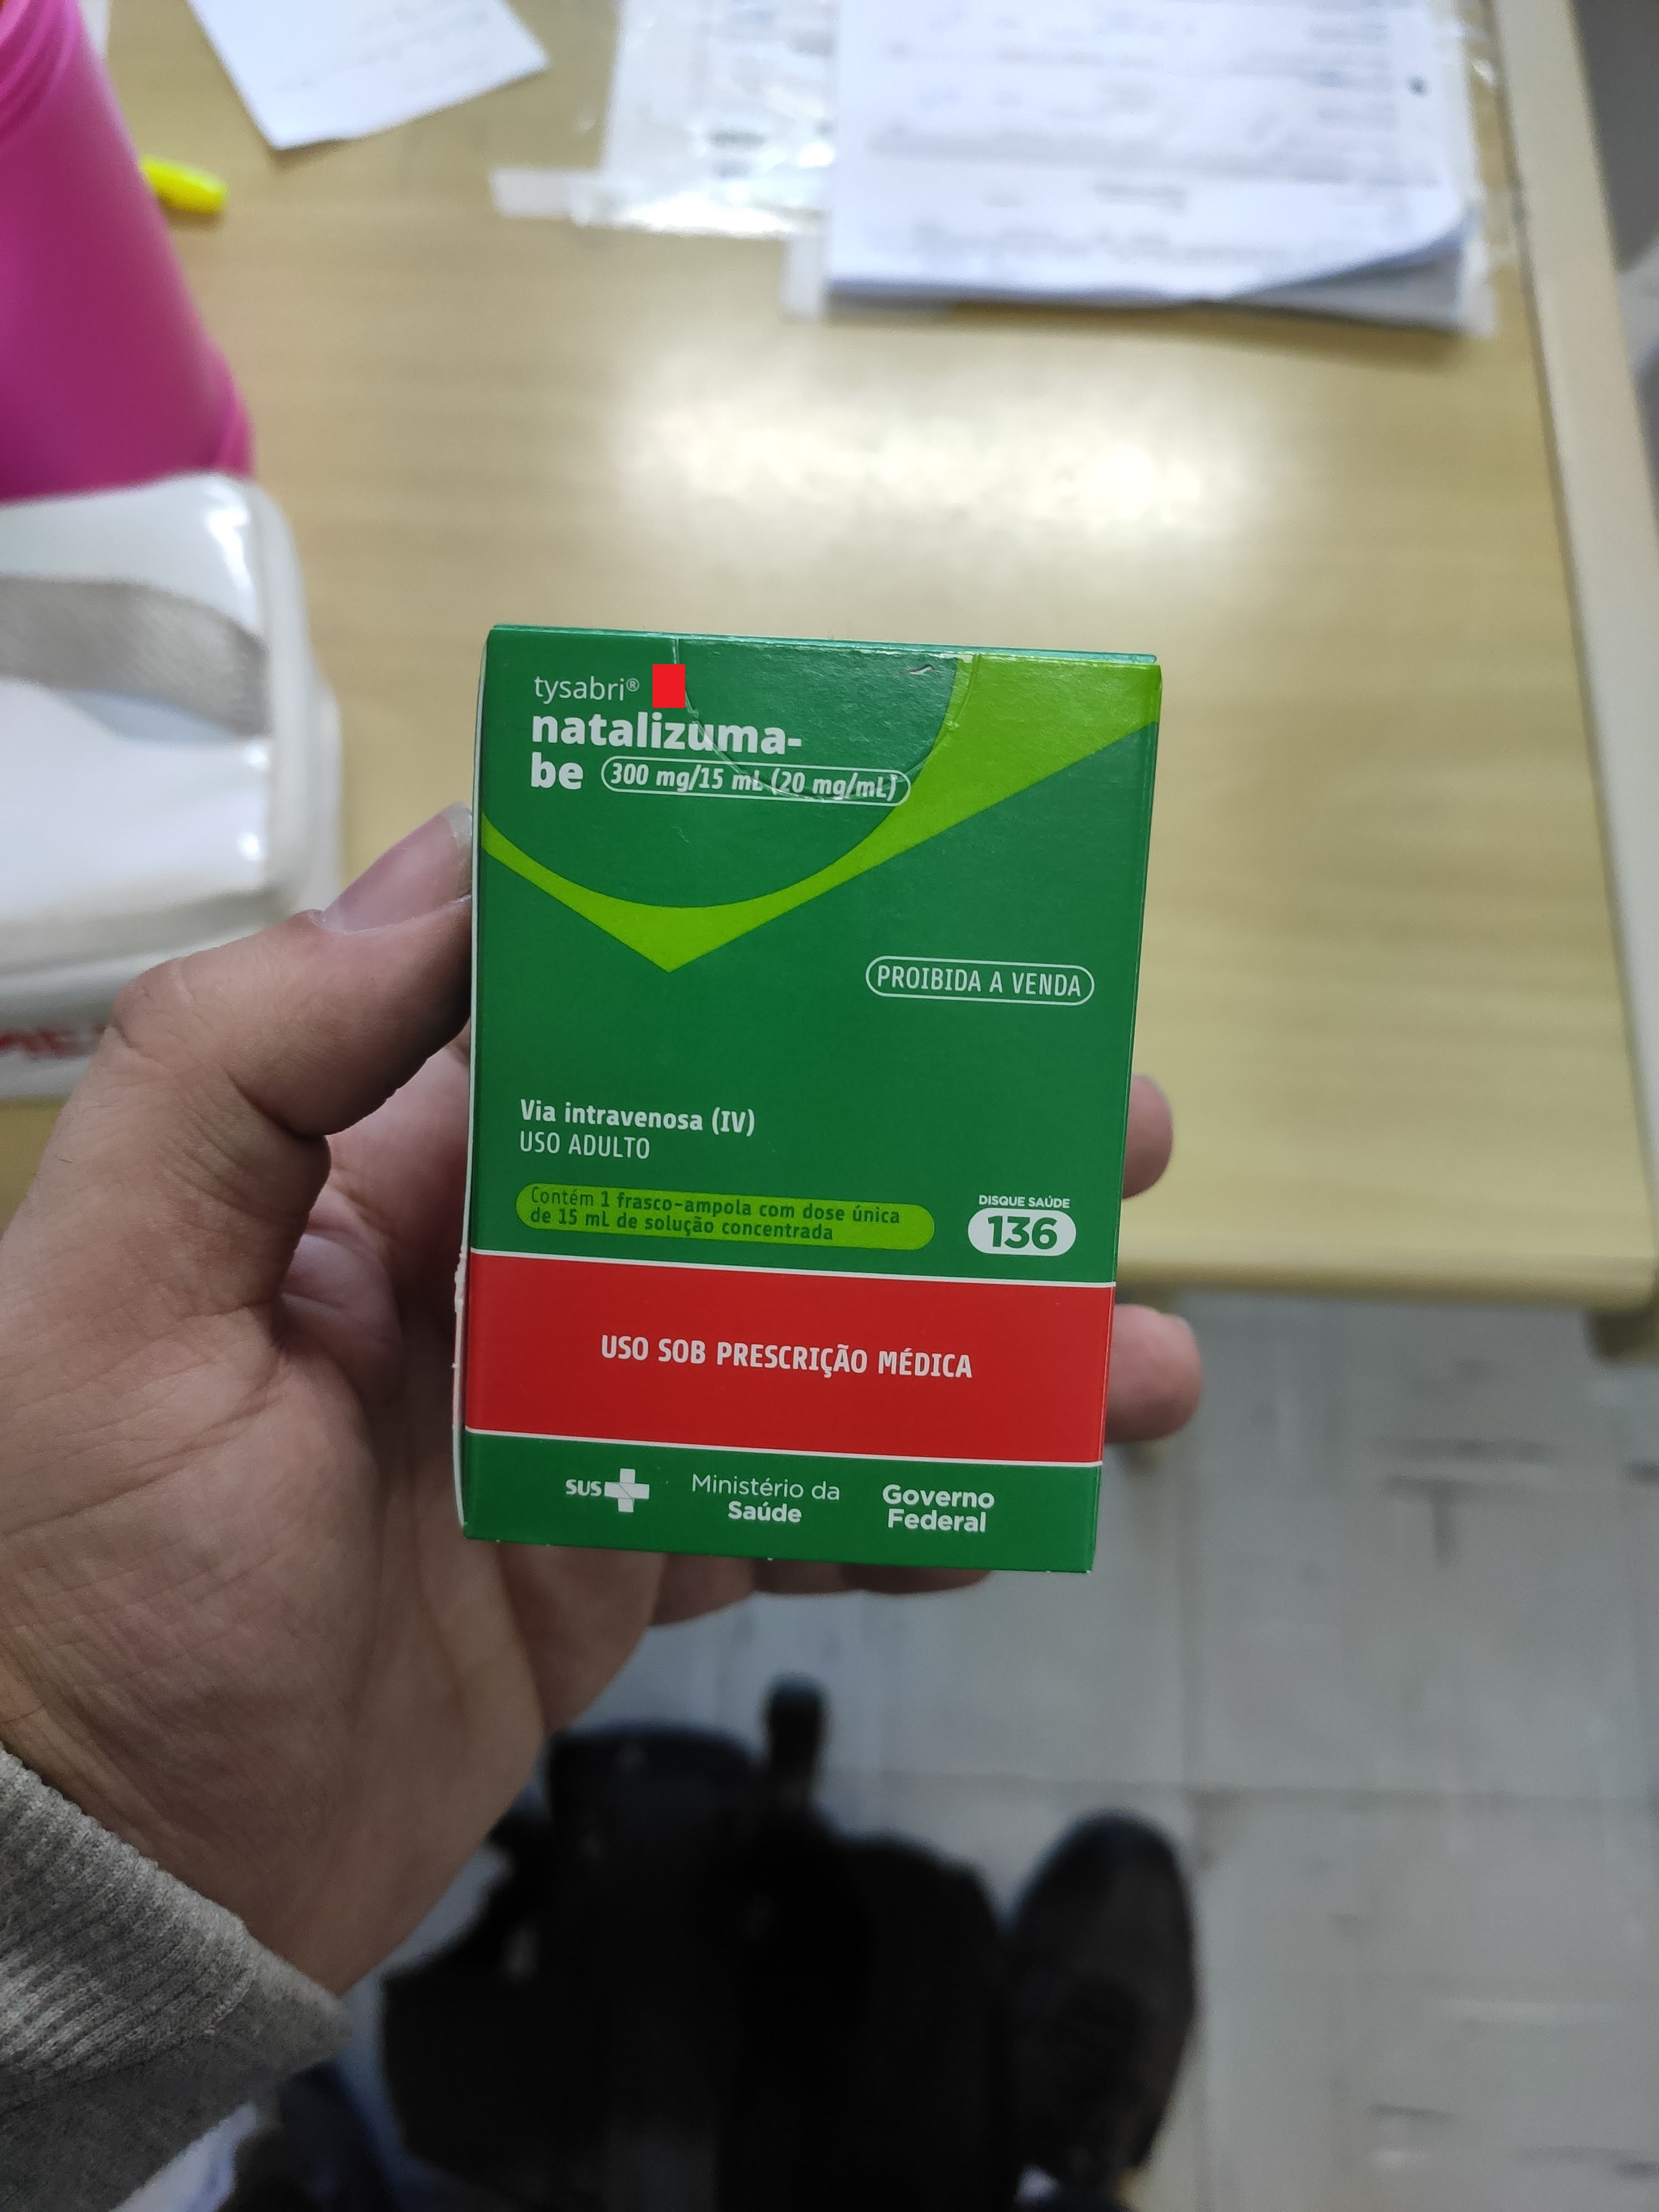
\includegraphics[width=\linewidth]{../pictures/tysabri.jpg}
        \caption*{Fonte: Autor.}
    \end{subfigure}
    \hfill
    \begin{subfigure}[t]{0.45\textwidth}
        \centering
        \caption{Recorte ao redor da área destacada.}
        \label{fig:fotos:tysabri_cortado}
        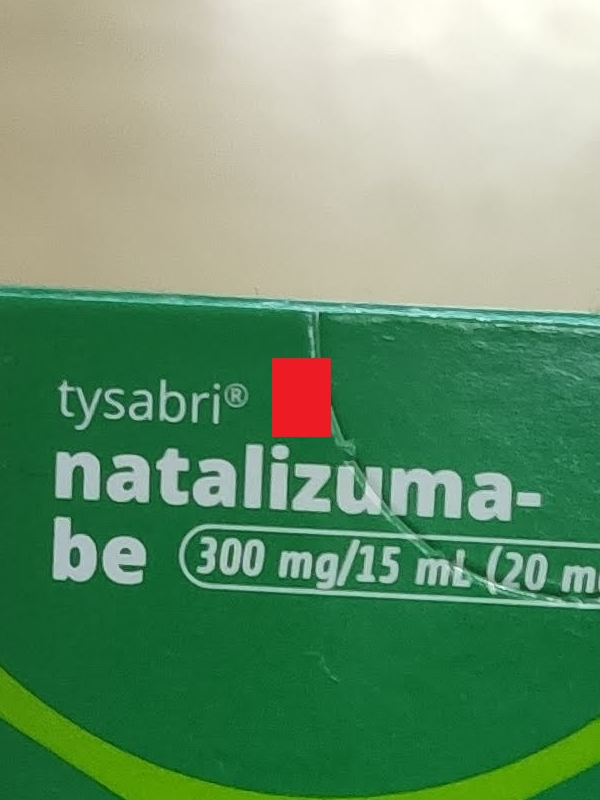
\includegraphics[width=\linewidth]{../pictures/tysabri cortado.jpg}
        \caption*{Fonte: Autor.}
    \end{subfigure}
    \hfill
    \label{fig:fotos:tamanho}
\end{figure}


\begin{lstfloat}[htbp]
    \centering
    \lstinputlisting[label=cod:ler:2, caption={Filtrar termos lidos, simplificado.}]{../code/ex_ler_2.py}
    \caption*{Fonte: Autor.}
\end{lstfloat}

\subsection{Gerar diferentes versões de imagem}\label{ssec:versoes}

Além da análise realizada na versão codificada em \ac{RGB} da imagem, também são analisadas variantes em codificação de cores nessa imagem, além da versão em escala de cinza.
Para cada codificação, são analisadas suas componentes separadamente.
Caso duas componentes encontrem palavras iguais, é mantida na lista a versão com maior valor de confiabilidade.

Em cada componente analisada, é aplicado um método de limiar para binarização dos valores.
As componentes binarizadas são utilizadas para recompor a imagem completa da codificação em questão e essa nova versão também é analisada.

As codificações analisadas foram:
\begin{itemize}
    \item \ac{RGB};
    \item \ac{CMYK};
    \item HLS;
    \item HSV;
    \item YCrCb.
\end{itemize}

A conversão para as versões HLS, HSV e YCrCb foi realizada através da função \lstinline|cvtColor|, da biblioteca de processamento de imagem \textit{OpenCV}, essa função converte a codificação de cores utilizada na imagem \cite{CV2cvtColor}.
A versão \ac{CMYK} é convertida utilizando as equações pertinentes.

A binarização por limiar das componentes é realizada pela função \textit{threshold}, da biblioteca de processamento de imagem \textit{OpenCV}, utilizando o método de Otsu \cite{CV2threshold}.
O \autoref{cod:versoes} apresenta uma simplificação da estrutura utilizada.


\begin{lstfloat}[htbp]
    \centering
    \lstinputlisting[label=cod:versoes, caption={Gerar versões das imagens, simplificado.}]{../code/ex_versoes.py}
    \caption*{Fonte: Autor.}
\end{lstfloat}

Os termos encontrados são adicionados a uma única lista, é possível que o mesmo tempo seja localizado em versões diferentes de imagem. Neste caso, é escolhida a versão com maior parâmetro de confiabilidade.

Cada termo encontrado é normalizado para evitar problemas na busca, removendo caracteres especiais e símbolos que não sejam letras dos termos.
São separados os termos compostos por mais de uma palavra, separados por hífen ou por detalhes na grafia, como letras maiúsculas dividindo palavras.

\subsection{Ordenar e selecionar termos encontrados na imagem}\label{ssec:organizar}

Com a lista de termos encontrados na imagem, analisando todas as codificações descritas anteriormente, é necessário ordenar os termos para que possam ser buscados.

Alguns termos recebem versões alternativas, pois a grafia correta pode ter sido removida na normalização dos termos.
Palavras com ``cao'', são replicadas para versões com ``ção'', casos semelhantes são realizados para ``ão'', ``cê'' e ``áci''.
A \autoref{fig:fotos:melagriao} apresenta um exemplo de medicamento que só é encontrado no sistema da \ac{Anvisa} se buscado com a grafia correta.
O \autoref{cod:organiza} apresenta uma simplificação da estrutura responsável por corrigir os termos.

\begin{figure}[htb]
    \centering
    \caption{Medicamento MELAGRIÃO\textsuperscript{\tiny\textregistered}, registrado na \ac{Anvisa} com caracteres especiais.}
    \label{fig:fotos:melagriao}
    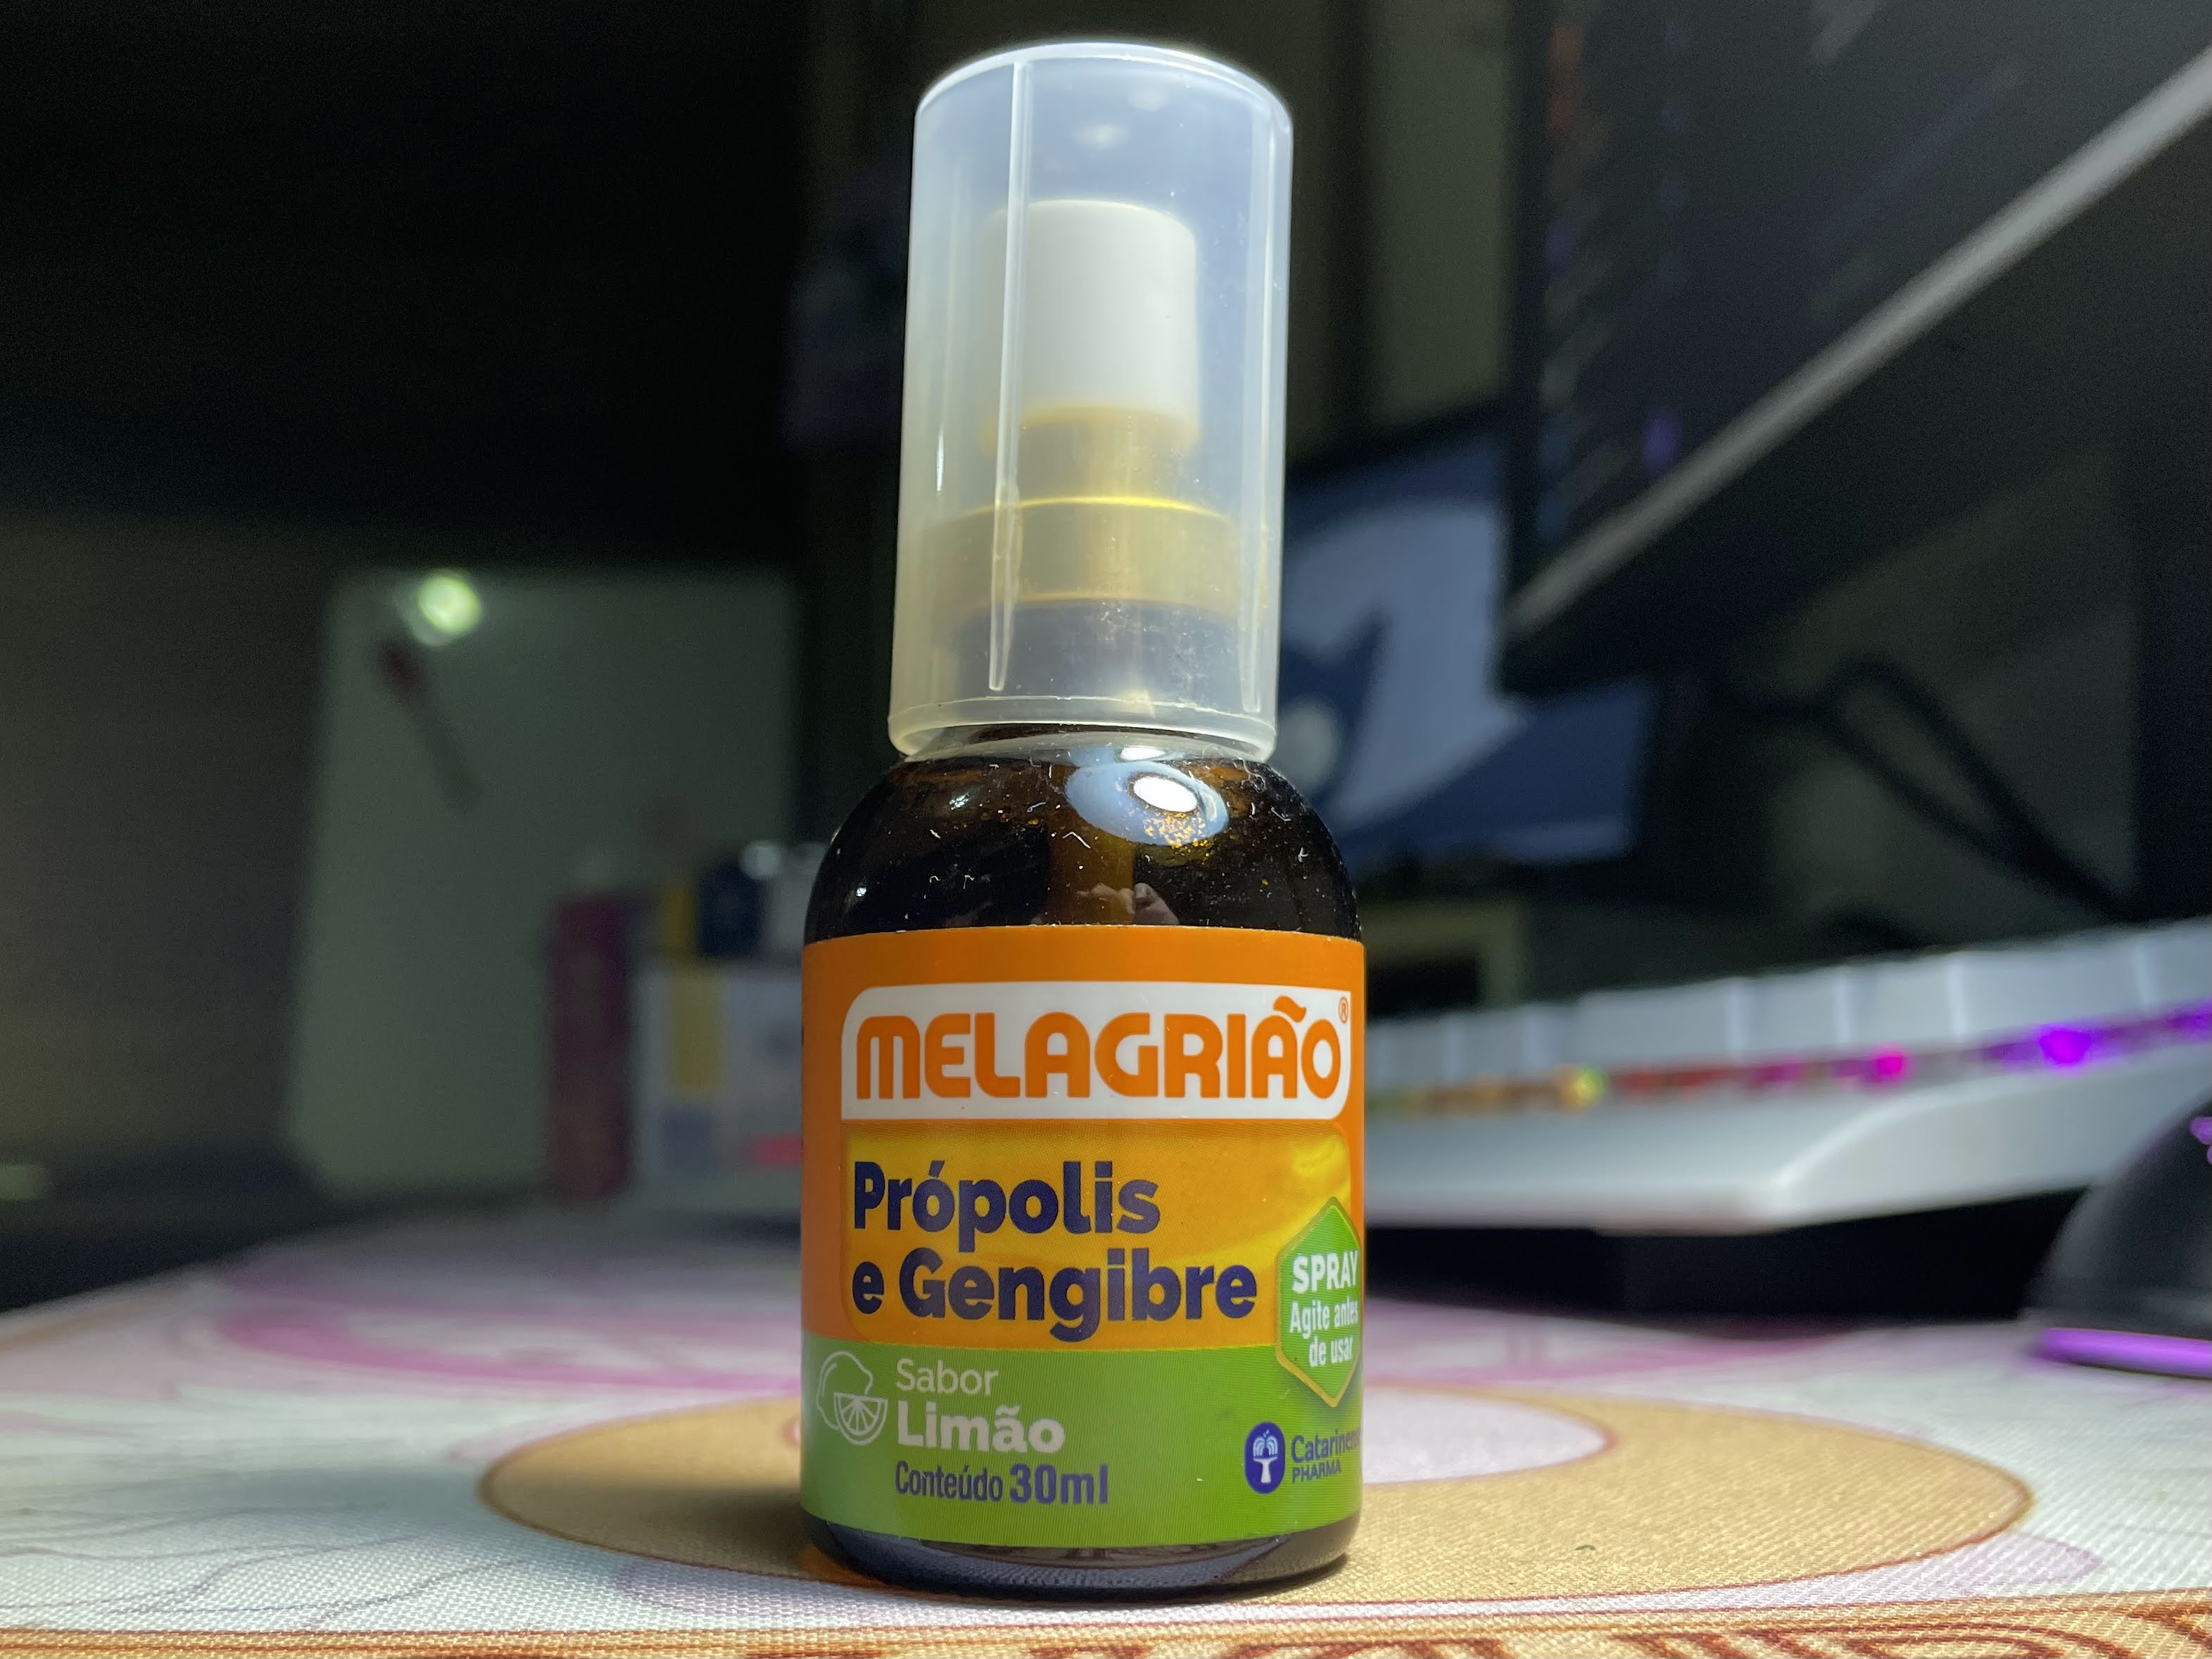
\includegraphics[width=0.45\linewidth]{../pictures/melagriao.jpg}
    \caption*{Fonte: Autor.}
\end{figure}


\begin{lstfloat}[htbp]
    \centering
    \lstinputlisting[label=cod:organiza, caption={Corrigir termos, simplificado.}]{../code/ex_organizar.py}
    \caption*{Fonte: Autor.}
\end{lstfloat}

O critério de ordenação utilizado é baseado nas características dos termos da lista.
São analisadas características como a escrita do termo, as propriedades do retângulo em que o termo está inscrito e o valor de confiabilidade fornecida pelo motor de \ac{OCR}, na seguinte ordem:
\begin{enumerate}
    \item Largura do retângulo na imagem pelo cálculo da divisão inteira por 10: $\left\lfloor \sfrac{w}{10} \right\rfloor$;
    \item Quantidade de caracteres do termo;
    \item Altura do retângulo na imagem pelo calculo da divisão inteira por 10: $\left\lfloor \sfrac{h}{10} \right\rfloor$;
    \item Posição vertical do centro do retângulo;
    \item Posição horizontal do centro do retângulo;
    \item Área do retângulo  na imagem pelo calculo da divisão inteira por 1000: $\left\lfloor \sfrac{A_{\text{termo}}}{1000} \right\rfloor$;
    \item Valor de confiabilidade do termo;
    \item Ordem lexicográfica do termo;
\end{enumerate}

A ordenação da lista de termos é realizada através do método \lstinline|sort| para listas, nativo da linguagem Python \cite{pythonSorting}, utilizando uma função de comparação com os critérios apresentados anteriormente.
O \autoref{cod:organiza:2} apresenta uma simplificação da estrutura responsável por ordenar os termos encontrados.

A ordem utilizada define quais serão os primeiros termos buscados no sistema do Bulário Eletrônico da \ac{Anvisa}.

\begin{lstfloat}[htbp]
    \centering
    \lstinputlisting[label=cod:organiza:2, caption={Ordenar termos, simplificado.}]{../code/ex_organizar_2.py}
    \caption*{Fonte: Autor.}
\end{lstfloat}

\subsection{Buscar no Bulário Eletrônica da \acs{Anvisa} os termos encontrados}\label{ssec:buscar}


Cada termo da lista é analisado antes da busca no Bulário Eletrônico da \ac{Anvisa}.
Termos com um único caractere são ignorados, porém são mantidos na lista pois podem fazer parte do nome do medicamento.

A busca de um termo no Bulário Eletrônico retorna uma lista com opções de medicamentos, neste contexto, chamados de possíveis candidatos.
É utilizado o método \lstinline|get| da biblioteca \textit{requests} \cite{reitz2024request}, que retorna um objeto contendo os dados da consulta.
Se a busca de um termo não retorna qualquer resultado, o próximo termo será buscado.
O \autoref{cod:buscar} apresenta uma simplificação de parte da estrutura utilizada.

\begin{lstfloat}[htbp]
    \centering
    \lstinputlisting[label=cod:buscar, caption={Buscar no Bulário Eletrônico, simplificado.}]{../code/ex_buscar.py}
    \caption*{Fonte: Autor.}
\end{lstfloat}

Além do nome do medicamente, a estrutura do candidato também apresenta informações pertinentes ao registro, como número de registro, data de emissão, identificação para o arquivo da bula eletrônica, razão social e \acs{CNPJ} da empresa responsável, entre outros.
A identificação para o arquivo da bula eletrônica poderá ser usado posteriormente na aquisição do arquivo pelo sistema.

Cada candidato tem seu nome analisado, normalizado e dividido em uma lista de palavras.
O primeiro critério de escolha um candidato baseia-se no termo utilizado na busca do Bulário Eletrônico, este termo deve ser encontrado na lista de palavras gerada pelo nome do medicamento.
Esse critério garante que partes de palavras comuns, como ``mono-'', não sejam suficientes para definir o nome de um remédio.

Atendido o critério, são conferidas as demais palavras da lista gerada pelo nome do candidato em questão.
Se a maioria das palavras existir na lista de termos, este candidato é considerado promissor.

Um candidato promissor é comparado ao melhor candidato encontrado até então, se a contagem de palavras correspondentes à lista de termos for maior, este candidato promissor se torna o melhor candidato.
Caso nenhum candidato seja considerado promissor, o próximo termo será analisado.

Se pelo menos um candidato dessa lista for considerador promissor, será retornado como escolhido para aquela imagem.

Caso um candidato seja escolhido, inicia-se o processo de carregamento do arquivo referente à bula eletrônica do medicamento.
O \autoref{cod:buscar:2} apresenta a continuação da versão simplificada da estrutura utilizada para a busca.

\begin{lstfloat}[htbp]
    \centering
    \lstinputlisting[label=cod:buscar:2, caption={Buscar no Bulário Eletrônico, simplificado.}]{../code/ex_buscar_2.py}
    \caption*{Fonte: Autor.}
\end{lstfloat}

% Cada nome será normalizado e dividido em suas palavras, e cada uma dessas palavras é buscada na lista de termos.

% O primeiro critério de escolha consiste em verificar se o termo buscado está na lista de palavras do nome atual.
% Esta verificação serve para garantir que termos comuns, como ``de'', não sejam suficientes para encontrar remédios erroneamente.

% Se o primeiro termo é encontrado com sucesso, as demais palavras do nome são buscadas na lista de termos.
% Define-se um melhor candidato dentre os encontrados quando a contagem de palavras coerentes é maior que a de palavras que não são encontradas.

% É possível que um nome de medicamente na lista fornecida pelo Bulário Eletrônico não possua candidatos elegíveis, neste caso, o seguinte nome da lista será analisado.



\subsection{Carregar o arquivo da bula do medicamento}\label{ssec:arquivo}

Utilizando a identificação para o arquivo da bula eletrônica, é possível construir o endereço web para requisitar este arquivo.
Novamente é utilizado o método \lstinline|get| da biblioteca \textit{requests} \cite{reitz2024request}, que retorna um objeto contendo os dados da requisição.

O conteúdo recebido é salvo em um arquivo local no formato \acs{PDF}, nomeado a partir do nome comercial do medicamento escolhido.
Este arquivo é criado utilizando o função \lstinline|open|, nativa da linguagem Python \cite{pythonOpen}, retornando um objeto da classe \lstinline|file|.
Este objeto fornece acesso ao arquivo aberto, no modo de escrita binária.

A escrita no arquivo é realizada utilizando o método \lstinline|write| para objetos da classe \lstinline|file|, nativo da linguagem Python \cite{pythonWrite}, atribuindo para o arquivo todo o conteúdo da requisição web feita anteriormente.
O \autoref{cod:carregar} apresenta uma simplificação da estrutura utilizada.

\begin{lstfloat}[htbp]
    \centering
    \lstinputlisting[label=cod:arquivo, caption={Carregar arquivo, simplificado.}]{../code/ex_arquivo.py}
    \caption*{Fonte: Autor.}
\end{lstfloat}


\subsection{Tratamento de erros e problemas de acesso}

Ao realizar uma requisição web, existe a chance de ocorrer um erro, seja por falha de conexão, tempo de resposta expirado, erros no HTTP, entre outros, estes erros lançam uma exceção pela classe \lstinline|requests| \cite{reitz2024request}.
Para lidar com estas exceções, é utilizada a estrutura \lstinline|try ... except ... finally| do Python \cite{refsnesdata2024, stack2013tryrequest}.

Nos casos pertinentes, o sistema irá fazer uma pausa de \num{10} segundos e tentar repetir a solicitação web.
Até \num{5} tentativas serão realizadas.
Caso o erro persista, após as tentativas de conexão, o sistema exibirá que houve um erro de conexão de seguirá com a execução.

No caso da consulta ao sistema do bulário eletrônico, a persistência do erro resulta num comportamento equivalente ao caso onde o termo buscado não retorna resultados.
Já no caso do carregamento do arquivo da bula, na persistência do erro, é exibida uma mensagem de erro, informando sobre o problema, e nenhum arquivo será salvo.
O \autoref{cod:try} apresenta a simplificação da estrutura utilizada.

% https://stackoverflow.com/questions/16511337/correct-way-to-try-except-using-python-requests-module
% https://www.w3schools.com/python/python_try_except.asp
% https://www.geeksforgeeks.org/try-except-else-and-finally-in-python/

\begin{lstfloat}[htbp]
    \centering
    \lstinputlisting[label=cod:try, caption={Modelo de estrutura \lstinline|try ... except ... finally| utilizado, simplificado.}]{../code/ex_try.py}
    \caption*{Fonte: Autor.}
\end{lstfloat}
